\section{The Incremental Algorithm}
\label{sec:algo}
To address these problems, we extended \learnpads{} to work incrementally.  
Given a candidate description \cd{D}, the new algorithm uses \cd{D} to parse
the records in the data source.  
It discards records that parse successfully, since these records are
already covered by \cd{D}, but it collects records that fail to parse.
When the algorithm accumulates $M$ such records, where $M$ is a
parameter of the algorithm, it invokes the incremental learning step,
described below, to produce a refined description \cd{D'}.  This refined
description subsumes \cd{D} and describes the $M$
new records.  In addition, the algorithm attempts to preserve as much
of the structure of \cd{D} as possible, so users supplying initial
descriptions can recognize the resulting descriptions. 
The algorithm then takes \cd{D'}
to be the new candidate description and repeats the process until it
has consumed all the input data.
The initial description \cd{D} can either be supplied by a user or it
can be inferred automatically by applying the original algorithm to
$N$ records selected from the data source, where $N$ is another
parameter.  
%Currently, the system selects a mix of $N/3$ consecutive lines
%taken from the beginning, middle, and end of the data source. 


Intuitively, the incremental learning step works by attempting to
parse each of the $M$ records according to the current description
\cd{D}.  It discards the portions of each record that parse correctly.
If a portion fails to parse, that failure will be detected at a
particular node in the description \cd{D}. It collects these failed
portions in an aggregation data structure \cd{A} that mirrors the
structure of \cd{D}.  After thus aggregating all the failures in the $M$
records, the algorithm transforms \cd{D} to accommodate the places where
differences were found (\ie, by introducing options where a piece of
data was missing or unions where a new type of data was discovered).
It then uses the original \learnpads{} algorithm to infer descriptions
for the aggregated portions of bad data. 

\figref{fig:data-structures} defines
the data structures for  descriptions \cd{D}, data
representations \cd{R}, and aggregate structures \cd{A}.
%
\begin{figure}[t]
{\small 
\begin{code}
\kw{Descriptions}:
Base ::= Pint | PstringME(re)
D ::=   
  Base             (Base token)
| Sync s           (Synchronizing token) 
| Pair (D\_1, D\_2)    (Pair)
| Union (D\_1, D\_2)   (Union)
| Array(D, s, t)   (Array)
| Option D         (Option)

\kw{Data representation}:
BaseR ::= Str s | Int i | Error
SyncR ::= Good | Fail | Recovered s 
R ::=
  BaseR
| SyncR
| PairR (R\_1, R\_2)
| Union1R R | Union2R R 
| ArrayR (R list, SyncR list, SyncR)
| OptionR R

\cdmath
\kw{Aggregation structure}:
A :: = 
  BaseA Base
| SyncA s
| PairA(A\_1, A\_2)
| UnionA(A\_l, A\_r)
| ArrayA (A\_elem, A\_sep, A\_term)
| OptionA A
| Opt A
| Learn [s]
\end{code}
\vskip -2ex
}
\caption{Data structures used in incremental inference}
\label{fig:data-structures}
\end{figure}
%
In these definitions,  variable \cd{re} ranges over regular expressions,
\cd{s} and \cd{t} over strings, and \cd{i} over integers.
A value with type \cd{D} is the abstract syntax tree of \pads{}
description: it is what we want to learn.  
For simplicity of presentation, we assume just two base types: 
integers and strings that match a regular expression. Synchronizing
tokens, or {\em sync tokens} for short, correspond to string literals
in \pads{} descriptions.  Such tokens, which are often
white space or punctuation,
serve as delimiters in the data and are useful for detecting
errors. We use binary pairs and unions to account for the
\kw{Pstruct}s and \kw{Punion}s in \padsc{} descriptions.
An array has an element type described by \cd{D}, a separator
string $s$ that appears between array elements, and a
terminator string $t$. \cd{Option D} indicates \cd{D} is optional.

A term with type \cd{R} is a parse tree obtained from parsing 
data using a description \cd{D}.  Parsing a base type can result in a
string, an integer or an error.  Parsing a sync token
\cd{Sync s} can give three different results: \cd{Good}, meaning the
parser found \cd{s} at the beginning of the input; \cd{Fail}, meaning
\cd{s} is not a substring of the current input; or \cd{Recovered s'},
meaning \cd{s} is not found at the beginning of the input, but
can be {\em recovered} after ``skipping'' string \cd{s'}.  The parse
of a pair is a pair of representations, and the parse of a union is
either the parse of the first branch or the parse of the second
branch. The parse of an array includes a list of parses for the
element type, a list of parses for the separator and a parse for the
terminator which appears at the end of the array.

An aggregate structure is the {\em accumulation} of parse trees; it
collects the data that cannot be parsed and therefore must be re-learned.
The aggregation structure mirrors the structure of the description \cd{D} 
with two additional nodes: an \cd{Opt} node, and a \cd{Learn} node. 
An invariant is that an \cd{Opt} node always wraps a \cd{BaseA} or a \cd{SyncA} node,
where it indicates that the underlying base or sync token is missing
in some of the parses being aggregated, and therefore that the wrapped
token should be made optional. 
%Note the difference between {\tt Opt} nodes and {\tt OptionA} nodes. The latter 
%just corresponds to the description {\tt Option D}. 
The \cd{Learn} node accumulates the bad portions of the data that need
to be learned. The newly learned sub-descriptions 
will be spliced into the original description to get the new description. 

\begin{figure}[t]
\begin{codebox}
incremental_step(d, xs) =
  as = [\kw{init_aggregate}(d)];
  foreach x in xs \{
    rs = \kw{parse}(d, x);
    as' = [];
    foreach r in rs \{
      foreach a in as \{
        a' = \kw{aggregate}(a, r); 
        as' = a :: as'
      \}
    \}
    as = as'
  \} 
  best_a = \kw{select_best}(as);
  d' = \kw{update_desc}(d, best_a);  
  return d'
\end{codebox}
\caption{Pseudo-code for the incremental learning step}
\label{fig:inc-learning}
\end{figure}

\figref{fig:inc-learning} gives pseudo-code for the incremental
learning step.
The \cd{init\_aggregate} function initializes an empty aggregate
according to description \cd{d}.  
Then for each data record \cd{x}, we use the \cd{parse} function to
produce a list \cd{rs} of possible parses.
We then call the \cd{aggregate} function to merge
each parse \cd{r} in the current list of parses with each aggregate \cd{a} in the
current list of aggregates. We use `\cd{::}' to denote 
consing an element onto the front of a list. 
When we finish
parsing all the data lines and obtain a final list of aggregates \cd{as}, we select
the best aggregate according to some criterion, and finally update the previous description
\cd{d} to produce the new description \cd{d'} using the best aggregate. 

\begin{figure}[t]
\begin{center}
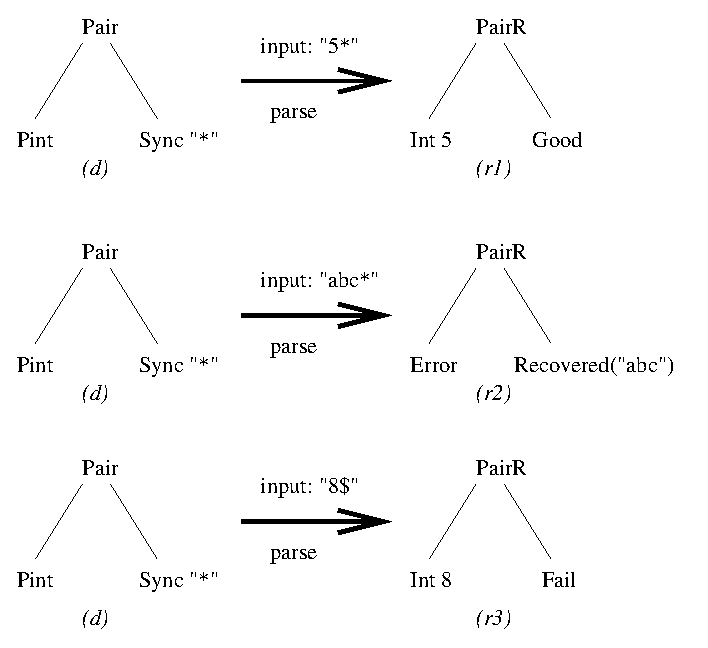
\epsfig{file=parse.eps, width=0.8\columnwidth}
\vskip -2ex
\caption{Result of parsing three input lines}\label{fig:parse}
\end{center}
\end{figure}

\begin{figure*}[t]
\begin{center}
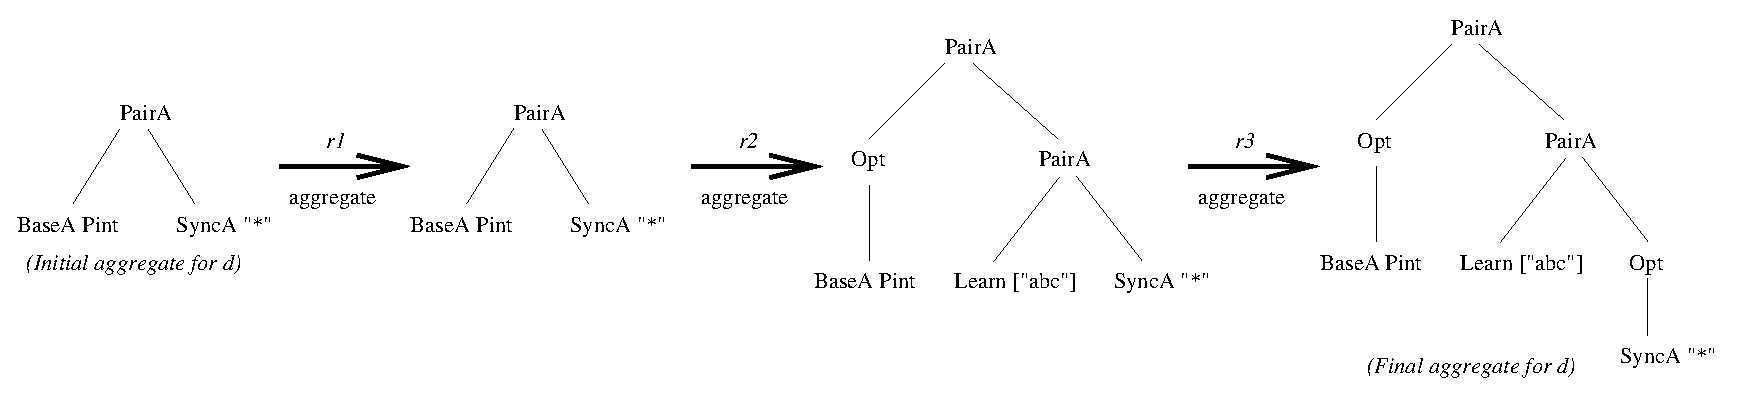
\epsfig{file=aggregate.eps, width=2\columnwidth}
\vskip -4ex
\caption{Aggregation of three parses}\label{fig:aggregate}
\end{center}
\end{figure*}

To illustrate the parsing and aggregation phases of the algorithm, we
introduce a simple example.
Suppose we have a description $d$, comprised of a pair of an integer and a sync token ``\cd{*}'',
and we are given the following three lines of new input:

{\small
\vskip -3.5ex
\begin{verbatim}
5*
abc*
8$
\end{verbatim}
\vskip -1ex
}
%
\noindent
\figref{fig:parse} shows the three data representations that result
from parsing the lines, which we call $r_1$, $r_2$ and $r_3$,
respectively. Notice the first line parsed without errors, the second
line contains an error for \cd{Pint} and some unparsable data ``{\tt
  abc}'', and the third contains a \cd{Fail} node because the
sync token \cd{*} was missing.  \figref{fig:aggregate} shows the aggregation
of $r_1$ to $r_3$ starting from an empty aggregate. In
general, \cd{Error} and \cd{Fail} nodes in the data representation
trigger the creation of \cd{Opt} nodes in the aggregate, while
unparsable data is collected in \cd{Learn} nodes.

\cut{
Parsing a union involves attempting to parse the first branch and, 
if it has error, attempting the second branch. This type of union semantics 
is known as {\em deterministic choice}, as opposed to a non-deterministic
choice where both branches are always attempted. 
When parsing an array, we use {\em longest match} semantics,
which means the parsing of the array elements and separators
continues until no more progress can be made in
the input. We will not elaborate these semantics because of lack of space.
}

%\begin{codebox}
%parse_all (d, x) =
%  switch (d) \{
%    case Pint =>  
%      (s, remainder) := match_prefix(x, "[0-9+\-]+");
%      if s != "" then return (Int s, remainder)
%      else return [(Error, x)];
%    case PstringME(re) => 
%      (s, remainder) := match_prefix(x, re);
%      if s != "" then return (Str s, remainder)
%      else return [(Error, x)];
%    case Sync s => 
%      (s', prefix, remainder) := match(x, s);
%      if s' = s and prefix = "" then return (Good, remainder)
%      elseif s' = "" then return (Fail, remainder)
%      else return [(Recovered prefix, remainder)]
%    case (x:d1, d2) =>
%      rs1 := parse_all (d1, x);
%      rs2 := [];
%      foreach (r1, remainder) in rs1 \{
%        (r2, remainder2) := parse_all (d2, remainder);
%        rs2 := rs2 + [((r1, r2), remainder2)]
%      \}
%    case (d1 + d2) => 
%	parse_all(d1, x) @ parse_all(d2, x)
%    case d array(sep, term) =>
%  \} 
%\end{codebox}    
%

\cut{%%%%%%%%%%%%%%%%%%%%%%%%%%%%%%%%

The {\tt parse\_all} function takes a description $d$ and an input string $x$, and returns
a list of all possible parses along with their respective ending position in the input. 
This function implements a standard recursive descent parser which recursively matches the
description structure (and sub-structures) with the input. To parse a pair $x: d_1 * d_2$, 
we first call {\tt parse\_all} on $d_1$ and get a list of parses. 
And then for each of the parse $r_1$ and corresponding end position, we bind $x$ to $r_1$ in
a private environment and  parse $d_2$ to get parses $l_2$. 
Finally for each parse $r_2$ in $l_2$ and each parse $r_1$ in $l_1$, 
construct a representation $(r_1, r_2)$, and return a list of all such pairs.
To parse a union $d_1 + d_2$, we simply return the concatenation of list of parses from
parsing $d_1$ and the list of parses from parsing $d_2$. To parse $d~ array(s, t)$,
we repeatedly attempt to parse $d$ until there's no more progress in the input.
And in each iteration, we also add parses generated from parsing $t$ as well, as if
the array has been terminated at this iteration. Figure \ref{fig:parse_base}
shows the {\tt parse\_base} function which parses a base token. The {\tt match\_prefix}
function matches the prefix of an input string with a regular expression and returns
the matched string and the remainder in the input. The {\tt match} function looks for
the first match of $s$ in input $x$, and returns the matched string $s'$, the prefix string
in $x$ before $s'$, and the remainder in the input.

\begin{figure}[t]
\begin{codebox}
parse_base (b, x) =
  switch (b) \{
  case Pint => 
    (s, suffix) := match_prefix(x, "[0-0+\-]+");
    if s <> "" then return [(Int s, suffix)];
    else return [(Error, x)]
  case PstringME(re) => 
    (s, suffix) := match_prefix(x, re);
    if s <> "" then return [(Str s, suffix)];
    else return [(Error, x)];
  case Sync s => 
    (s', prefix, remainder) := match(x, s);
    if s' = s and prefix = "" then 
      return (Good, remainder)
    elseif s' = "" then 
      return (Fail, remainder)
    else return [(Recovered prefix, remainder)]
  \}
\end{codebox}
\caption{Function to parse a base token or a sync token} \label{fig:parse_base}
\end{figure}

As an example, let $d$ be {\tt (Pint, Sync "|") + (PstringME "[a-z]+", Sync "|")}, 
and $x$ be ``\verb#abc|#''. {\tt parse\_all(d, x)} gives the following two possible parses:
{\small
\begin{verbatim}
  inl (Error, Recovered "abc")
  inr (Str "abc", Good)
\end{verbatim}
}

The {\tt aggregate} function adds a parse into an existing aggregate structure. When there is
no errors in the parse, it makes no changes to the aggregate. If the parse contains 
an error or failure for parsing token $b$, then the aggregate component 
$b$ is transformed to $opt~ b$, to indicate that $b$ node is optional. 
If a parse contains a recovered data $Recovered~ r$, then
a optional learn node will be created before the sync node. And the new aggregate component will be
$(opt (l [r]),~ Sync~ s)$. If the aggregate structure already contains the learn node before this
sync node, then recovered data $r$ will be added to the list under $l$.

The {\tt select\_best} function computes a score by counting the total number of $opt$ and $l$ nodes
in each of the aggregates, and returns the one with the smallest number. The idea is that the
aggregate with the smallest number of added nodes is more likely to represent a new description
that is the closest to the original description. 

Finally, the {\tt update\_desc} function does two things. First, it invokes the format inference
algorithm to learn a sub-description for the data strings collected at each of the learn nodes
and replace the learn nodes with these new sub-descriptions. Then, it uses a number of rewriting
rules into improve the overall structure. We will discuss some of these rewriting rules in more
details in section \ref{sec:imp}.

}%%%%%%%%%%%%%%%%%%%%%%%%%%%%%%%%% END OF CUT %%%%%%%%%%%%%%%%

% - problem definition (as close to the previous description as possible) (but we don't
%   have a metric to measure how close yet, do we want to mention tree edit distance??)
% - overview of algorithm: parsing + aggregating + rewriting
% - parsing algo (parse rep, score metric, pseudo-code)
% - aggregating algo (in pseudo code)
% - selection of top aggregates
% - update original description
% - rewriting rules (data independent, data dependent, OptsTable)

